\documentclass[10pt]{article}
\usepackage[utf8]{inputenc}
\usepackage{geometry}
\usepackage[sort]{natbib}
\usepackage{pxfonts}
\usepackage{graphicx}
\usepackage{setspace}
\usepackage{hyperref}
\usepackage{lineno}
\usepackage{authblk}

\doublespacing
\linenumbers

\title{Fitness tracking reveals task-specific associations between
  memory, mental health, and exercise}
\author[1, $\star$]{Jeremy R. Manning}
\author[1,2]{Gina M. Notaro}
\author[1]{Esme Chen}
\author[1]{Paxton C. Fitzpatrick}
\affil[1]{Dartmouth College, Hanover, NH}
\affil[2]{Lockheed Martin, Bethesda, MD}
\affil[$\star$]{Address correspondence to
  jeremy.r.manning@dartmouth.edu}


\newcommand{\devices}{S1}
\newcommand{\frDetail}{S2}
\newcommand{\natDetail}{S3}
\newcommand{\vocabDetail}{S4}
\newcommand{\spatialDetail}{S5}
\newcommand{\fitDists}{S6}
\newcommand{\fitDistgridImmediate}{S7}
\newcommand{\fitScatterImmediate}{S8}
\newcommand{\fitDistgridDelayed}{S9}
\newcommand{\fitScatterDelayed}{S10}
\newcommand{\behBehCorr}{S11}
\newcommand{\fitFitCorr}{S12}
\newcommand{\demDemCorr}{S13}
\newcommand{\allCorr}{S14}


\begin{document}
\maketitle

\begin{abstract}
  Physical exercise can benefit both physical and mental well-being.
  Different forms of exercise (i.e., aerobic versus anaerobic; running
  versus walking versus swimming versus yoga; high-intensity interval
  training versus endurance workouts; etc.) impact physical fitness
  in different ways.  For example, running may substantially impact
  leg and heart strength but only moderately impact arm strength. We
  hypothesized that the mental benefits of exercise might be similarly
  differentiated.  We focused specifically on how different forms of
  exercise might related to different aspects of memory and mental
  health.  To test our hypothesis, we collected nearly a century's
  worth of fitness data (in aggregate).  We then asked participants to
  fill out surveys asking them to self-report on different aspects of
  their mental health.  We also asked participants to engage in a
  battery of memory tasks that tested their short and long term
  episodic, semantic, and spatial memory.  We found that participants
  with similar exercise habits and fitness profiles tended to also
  exhibit similar mental health and task performance profiles.
\end{abstract}

\section*{Introduction}
Engaging in physical activity (exercise) can improve our physical
fitness by increasing muscle strength~\citep{RogeEvan93, Lind79,
  CranEtal13, Knut07}, increasing bone density~\citep{ChilEtal12,
  BassRams94, LaynNels99}, increasing cardiovascular
performance~\citep{MaioEtal00, PollEtal00}, increasing lung
capacity~\citep{LazoEtal16}~\citep[although see][]{RomaEtal16},
increasing endurance~\citep{WilmKnut03}, and more.  Exercise can also
improve mental health~\citep{Ragl90, MikkEtal17, TaylEtal85,
  DeslEtal09, Call04, PaluSchw00, BassSuzu17} and cognitive performance~\citep{ChanEtal12b,
  BrisEtal02, EtniEtal06, BassSuzu17}.

The physical benefits of exercise can be explained by stress-responses
of the affected body tissues. For example, skeletal muscles that are
taxed during exercise exhibit stress responses~\citep{MortEtal09} that
can in turn affect their growth or atrophy~\citep{SchiEtal13}.  By
comparison, the benefits of exercise on mental health are less direct.  For
example, one hypothesis is that exercise leads to specific
physiological changes, such as increased aminergic synaptic
transmission and endorphin release, which in turn act on
neurotransmitters in the brain~\citep{PaluSchw00}.

Speculatively, if different exercise regimens lead to different
neurophysiological responses, one might be able to map out a spectrum
of signalling and transduction pathways that are impacted by a given
type, duration, and intensity of exercise in each brain region.  For
example, prior work has shown that exercise increases acetylcholine
levels, starting in the vicinity of the exercised
muscles~\citep{ShoeEtal97}.  Acetylcholine is thought to play an
important role in memory formation~\citep[e.g., by modulating specific
synaptic inputs from entorhinal cortex to the hippocampus, albeit in
rodents;]{PalaEtal21}.  Given the central role of these medial
temporal lobe structures play in memory, changes in acetylcholine
might lead to specific changes in memory formation and retrieval.

In the present study, we hypothesize that (a) different exercise regimens will
have different, quantifiable impacts on cognitive performance and
mental health, and that (b) these impacts will be consistant across
individuals.  To this end, we collected a year of fitness tracking
data from each of 113 participants.  We then asked each participant to
fill out a brief survey in which they self-evaluated several aspects
of their mental health.  Finally, we ran each participant through a
battery of memory tasks, which we used to evaluate their memory
performance along several dimensions.  We examined the data for
potential associations between memory, mental health, and exercise.

 \section*{Methods}

    We ran an online experiment using the Amazon Mechanical Turk
    platform.  We collected data about each participant's fitness and
    exercise habits, a variety of self-reported measures concerning their
    mental health, and about their performance on a battery of memory
    tasks.  We mined the dataset for potential associations between
    memory, mental health, and exercise.

    
    
\subsection*{Experiment}
\subsubsection*{Participants}
We recruited experimental participants by posting our experiment as a
Human Intelligence Task (HIT) on the Amazon Mechanical Turk platform.
We limited participation to Mechanical Turk Workers who had been
assigned a ``Masters'' designation on the platform, given to workers
who score highly across several metrics on a large number of HITs,
according to a proprietary algorithm managed by Amazon.  We further
limited our participant pool to participants who self-reported that
they were fluent in English and regularly used a Fitbit fitness
tracker device.  A total of 160 workers accepted our
HIT in order to participate in our experiment.  Of these, we excluded all
participants who failed to log into their Fitbit account (giving us
access to their anonymized fitness tracking data), encountered
technical issues (e.g., by accessing the HIT using an incompatible browser, device, or
operating system), or who ended their participation prematurely,
before completing the full study.  In all, 113 participants remained
that contributed usable data to the study.

For their participation, workers received a base payment of \$5 per hour (computed in 15
minute increments, rounded up to the nearest 15 minutes), plus an
additional performance-based bonus of up to \$5.  Our recruitment
procedure and study protocol
were approved by Dartmouth's Committee for the Protection of Human Subjects.

\paragraph{Gender, age, and race.}
Of the 113 participants who contributed usable data, 77 reported their gender as female, 35 as
male, and 1 chose not to report their gender.  Participants ranged in
age from 19--68 years old (25\textsuperscript{th} percentile: 28.25
years; 50\textsuperscript{th} percentile: 32 years;
75\textsuperscript{th} percentile: 38 years).  Participants reported
their race as White (90 participants), Black or African American (11
participants), Asian (7 participants), Other (4 participants), and
American Indian or Alaska Native (3 participants).  One participant
opted not to report their race.

\paragraph{Languages.}
All participants reported that they were fluent in either 1 and 2
languages (25\textsuperscript{th} percentile: 1;
50\textsuperscript{th} percentile: 1; 75\textsuperscript{th}
percentile: 1), and that they were ``familiar'' with between 1 and 11
languages (25\textsuperscript{th} percentile: 1;
50\textsuperscript{th} percentile: 2; 75\textsuperscript{th}
percentile: 3).

\paragraph{Reported medical conditions and medications.}
Participants reported having and/or taking medications pertaining to the following medical conditions: anxiety or
depression (4 participants), recent head injury (2 participants), high
blood pressure (1 participant), bipolar (1 participant),
hypothyroidism (1 participant), and other unspecified medications (1
participant).  Participants reported their current and typical stress
levels on a Likert scale as very relaxed (-2), a little relaxed (-1),
neutral (0), a little stressed (1), or very stressed (2).  The
``current'' stress level reflected participants' stress at the time
they participated in the experiment.
Their responses
ranged from -2 to 2 (current stress: 25\textsuperscript{th} percentile: -2;
50\textsuperscript{th} percentile: -1; 75\textsuperscript{th}
percentile: 1; typical stress: 25\textsuperscript{th} percentile: 0;
50\textsuperscript{th} percentile: 1; 75\textsuperscript{th}
percentile: 1).  Participants also reported their current level of
alertness on a Likert scale as very sluggish (-2), a little sluggish
(-1), neutral (0), a little alert (1), or very alert (2).  Their
responses ranged from -2 to 2 (25\textsuperscript{th} percentile: 0;
50\textsuperscript{th} percentile: 1; 75\textsuperscript{th}
percentile: 2).  Nearly all (111 out of 113) participants reported
that they had normal color vision, and 15 participants reported
uncorrected visual impairments (including dyslexia and uncorrected
near- or far-sightedness).

\paragraph{Residence and level of education.}
Participants reported their residence
as being located in the suburbs (36 participants), a large city (30
participants), a small city (23 participants), rural (14
participants), or a small town (10 participants).  Participants
reported their level of education as follows: College graduate (42
participants), Master's degree (23 participants), Some college (21
participants), High school graduate (9 participants), Associate's
degree (8 participants), Other graduate or professional school (5
participants), Some graduate training (3 participants), or Doctorate
(2 participants).

\paragraph{Reported water and coffee intake.}
Participants reported the number of cups of water and coffee they had
consumed prior to accepting the HIT.  Water consumption ranged from
0--6 cups (25\textsuperscript{th} percentile: 1;
50\textsuperscript{th} percentile: 3; 75\textsuperscript{th}
percentile: 4).  Coffee consumption ranged from 0--4 cups (25\textsuperscript{th} percentile: 0;
50\textsuperscript{th} percentile: 1; 75\textsuperscript{th}
percentile: 2).


\subsubsection*{Tasks}
Upon accepting the HIT posted on Mechanical Turk, the worker was
directed to read and fill out a screening and consent form, and to
share access to their anonymized Fitbit data via their Fitbit account.
After consenting to participant and successfully sharing their Fitbit
data, participants filled out a survey and then engaged in a series of
memory tasks (Fig.~\ref{fig:tasks}).  All stimuli and code for running
the full Mechanical Turk experiment may be found
\href{https://github.com/ContextLab/brainfit-task}{\underline{here}}.

\begin{figure}[tp]
\centering
\includegraphics[width=1\textwidth]{figs/experiment}
\caption{\textbf{Battery of memory tasks.}  \textbf{a.  Free recall.}
Participants study 16 words (presented one at a time), followed by an
immediate memory test where they type
each word they remember from the just-studied list.  In the delayed
memory test, participants type any words they remember studying, from
any list.  \textbf{b. Naturalistic recall.}  Participants watch a
brief video, followed by two immediate memory tests.  The first test
asks participants to write out what happened in the video.  The second
test has participants answer a series of multiple choice questions
about the conceptual content of the video.  In the delayed memory
test, participants (again) write out what happened in the video.
\textbf{c. Foreign language flashcards.}  Participants study a
sequence of 10 English-Gaelic word pairs, each presented with an
illustration of the given word.  During an immediate memory test,
participants perform a multiple choice test where they select the
Gaelic word that corresponds to the given photograph.  During the
delayed memory test, participants perform a second multiple choice
test, where they select the Gaelic word that corresponds to each of a
new set of photographs.  \textbf{d. Spatial learning.}  In each trial,
participants
study a set of randomly positioned shapes.  Next, the shapes'
positions are altered, and participants are asked to drag the shapes
back to their previous positions.  \textbf{All panels.}  The gray
numbers denote the order in which participants experienced each task
or test.}
\label{fig:tasks}
\end{figure}

\paragraph*{Survey questions.}  We collected the following demographic
information from each participant: their birth year, gender, highest
(academic) degree achieved, race, language fluency, and language
familiarity.  We also collected information about participants'
health and wellness, including about their vision, alertness, stress, sleep, coffee
and water consumption, location of their residence, activity typically
required for their job, and exercise habits.


\paragraph*{Free recall (Fig.~\ref{fig:tasks}a).} 
Participants studied a sequence of four word lists, each comprising 16
words.  After studying each list, participants received an immediate
memory test, whereby they were asked to type (one word at a time) any
words they remembered from the just-studied list, in any order.

Words were presented for 2~s each, in black text on a white
background, followed by a 2~s blank (white) screen.  After the final
2~s pause, participants were given 90~s to type in as many words as
they could remember, in any order.  The memory test was constructed
such that the participant could only see the text of the current word
they were typing; when they pressed any non-letter key, the current
word was submitted and the text box they were typing in was cleared.
This was intended to prevent participants from retroactively editing
their previous responses.

The word lists participants studied were drawn from the categorized
lists reported in \cite{ZimaEtal18}.  Each participant was assigned
four unique randomly chosen lists (in a randomized order), selected
from a full set of 16 lists.  Each chosen list was then randomly
shuffled before presenting the words to the participants.

Participants also performed a final delayed memory test where they
were given 180~s to type out any words they remembered from
\textit{any} of the 4 lists they had studied.

Recalled words within an edit distance of 2 (i.e., a Levenshtein Distance less
than or equal to 2) of any word in the wordpool were ``autocorrected''
to their nearest match.  We also manually corrected clear typos or
misspellings by hand (e.g., we corrected ``hippoptumas'' to
``hippopotamus'', ``zucinni'' to ``zucchini'', and so on).  Finally,
we lemmatized each submitted word to match the plurality of the
matching wordpool word (e.g., ``bongo'' was corrected to ``bongos'',
and so on).  After applying these corrections, any submitted words
that matched words presented on the just-studied list were tagged as
``correct'' recalls, and any non-matching words were discarded as
``errors.''  Because participants were not allowed to edit the text
they entered, we chose not to analyze these putative ``errors,'' since
we could not distinguish typos from true misrememberings.

\paragraph*{Naturalistic recall (Fig.~\ref{fig:tasks}b).}
Participants watched a 2.5~minute video clip entitled ``The Temple of
Knowledge.''  The video comprises an animated story told to StoryCorps
by Ronald Clark, who was interviewed by his daughter, Jamilah Clark.
The narrator (Ronald) discusses growing up living in an apartment over
Washington Heights branch of the New York Public Library, where his
father worked as a custodian during the 1940s.

After watching the video clip, participants were asked to type out
anything they remembered about what happened in the video.  They typed
their responses into a text box, one sentence at a time.  When the
participant pressed the return key or typed any final punctuation mark
(``.'', ``!'', or ``?'') the text currently entered into the box was
``submitted'' and added to their transcript, and the text box was
cleared to prevent further editing of any already-submitted text.
This was intended to prevent participants from retroactively editing
their previous responses.  Participants were given up to 10~minutes to
enter their responses.  After 4~minutes participants were given the
option of ending the response period early, e.g., if they felt they
had finished entering all of the information they remembered.  Each
participant's transcript was constructed from their submitted
responses by combining the sentences into a single document and
removing extraneous whitespace characters.

Following this 4--10 minute free response period, participants were
given a series of 10 multiple choice questions about the conceptual
content of the story.  All participants received the same questions,
in the same order.

Participants also performed a final delayed memory test, where they
carried out the free response recall task a second time, near the end
of the testing session.  This resulted in a second transcript, for
each participant.

\paragraph*{Foreign language flashcards (Fig.~\ref{fig:tasks}c).}
Participants studied a series of 10 English-Gaelic word pairs in a
randomized order.  We selected the Gaelic language both for its
relatively small number of native speakers and for its dissimilarity
to other commonly spoken languages amongst Mechanical Turk Workers.
We verified (via self report) that all of our participants were fluent
in English and that they were neither fluent nor familiar with Gaelic.

Each word's ``flashcard'' comprised a cartoon depicting the given
word, the English word or phrase in lowercase text (e.g., ``the
boy''), and the Gaelic word or phrase in uppercase text (e.g.,
``BUACHAILL'').  Each flashcard was displayed for 4~s, followed by a
3~s interval (during which the screen was cleared) prior to the next
flashcard presentation.

After studying all 10 flashcards, participants were given a multiple
choice memory test where they were shown a series of novel
photographs, each depicting one of the 10 words they had learned.
They were asked to select which (of 4 unique options) Gaelic word went
with the given picture.  The 3 incorrect options were selected at
random (with replacement across trials), and the order in which the
choices appeared to the participant were also randomized.  Each of the
10 words they had learned were tested exactly once.

Participants also performed a final delayed memory test, where they
were given a second set of 10 questions (again, one per word they had
studied).  For this second set of questions participants were prompted
with a new set of novel photographs, and new randomly chosen incorrect
choices for each question.  Each of the 10 original words they had
learned were (again) tested exactly once during this final memory
test.



\paragraph*{Spatial learning (Fig.~\ref{fig:tasks}d).}
Participants performed a series of study-test trials where they
memorized the onscreen spatial locations of two or more shapes.
During the study phrase of each trial, a set of shapes appeared on the
screen for 10~s, followed by 2~s of blank (white) screen.  During the
test phase of each trial, the same shapes appeared onscreen again, but
this time they were vertically aligned and sorted horizontally in a
random order.  Participants were instructed to drag (using the mouse)
each shape to its studied position, and then to click a button to
indicate that the placements were complete.

In different study-test trials, participants learned the locations of
different numbers of shapes (always drawn from the same pool of 7
unique shapes, where each shape appeared at most one time per trial).
They first performed three trials where they learned the locations of
2 shapes; next three trials where they learned the locations of 3
shapes; and so on until their last three trials, where (during each
trial) they learned the locations of 7 shapes.  All told, each
participant performed 18 study-test trials of this spatial learning
task (3 trials for each of 2, 3, 4, 5, 6, and 7 shapes).


\subsubsection*{Fitness tracking using Fitbit devices}
To gain access to our study, participants provided us with access to
all data associated with their Fitbit account from the year (365
calendar days) up to and including the day they accepted the HIT.  We
filtered out all identifiable information (e.g., participant names,
GPS coordinates, etc.) prior to importing their data.

\subsubsection*{Collecting and processing Fitbit data}

The fitness tracking data associated with participants' Fitbit
accounts varied in scope and duration according to which device the
participant owned (Fig.~\devices), how often the participant
wore (and/or synced) their tracking device, and how long they had
owned their device.  For example, while all participants' devices
supported basic activity metrics such as daily step counts, only a
subset of the devices with heart rate monitoring capabilities provided
information about workout intensity, resting heart rate, and other
related measures.


Across all devices, we collected the following information: heart rate
data, sleep tracking data, logged bodyweight measurements, logged
nutrition measurements, Fitbit account and device settings, and
activity metrics.

\paragraph{Heart rate.}  If available, we extracted all heart rate
data collected by participants' Fitbit device(s) and associated with
their Fitbit profile.  Depending on the specific device model(s) and
settings, this included second-by-second, minute-by-minute, daily
summary, weekly summary, and/or monthly summary heart rate
information.  These summaries include information about participants'
average heart rates, and the amount of time they were estimated to
have spent in different ``heart rate zones'' (rest, out-of-range, fat
burn, cardio, or peak, as defined by their Fitbit profile), as well as
an estimate of the number of estimated calories burned while in each
heart rate zone.

\paragraph{Sleep.}  If available, we extracted all sleep data
collected by participants' Fitbit device(s).  Depending on the
specific device model(s) and settings, this included nightly estimates
of the duration and quality of sleep, as well as the amount of time
spent in each sleep stage (awake, REM, light, or deep).

\paragraph{Weight.}  If available, we extracted any weight-related
information affiliated with participants' Fitbit accounts within 1
year prior to enrolling in our study.  Depending on their specific
device model(s) and settings, this included their weight, body mass
index, and/or body fat percentage.

\paragraph{Nutrition.} If available, we extracted any
nutrition-related information affiliated with participants' Fitbit
accounts within 1 year prior to enrolling in our study. Depending on
their specific account settings and usage behaviors, this included a
log of the specific foods they had eaten (and logged) over the past
year, and the amount of water consumed each day.

\paragraph{Account and device settings.}  We extracted any settings
associated with participants' Fitbit accounts to determine (a) which
device(s) and model(s) are associated with their Fitbit account, (b)
time(s) when their device(s) were last synced, and (c) battery
level(s).

\paragraph{Activity metrics.}  If available, we extracted any
activity-related information affiliated with participants' Fitbit
accounts within 1 year prior to enrolling in our study.  Depending on
their specific device model(s) and settings, this included: daily step
counts; daily amount of time spent in each activity level (sedentary,
lightly active, fairly active, or very active, as defined by their
account settings and preferences); daily number of floors climbed;
daily elevation change; and daily total distance traveled.



\subsubsection*{Comparing recent versus baseline measurements.}
We were interested in separating out potential associations between
\textit{absolute} fitness metrics and \textit{relative} metrics.  To
this end, in addition to assessing potential raw (absolute) fitness
metrics, we also defined a simple measure of recent changes in those
metrics, relative to a baseline:
\[
  \Delta_{R, B} m = \frac{B \sum_{i = 1}^R
  m(i)}{R \sum_{i=R + 1}^{R+B}m(i)},
\]
where $m(i)$ is the value of metric $m$ from $i - 1$ days prior to
testing (e.g., $m(1)$ represents the value of $m$ on the day the
participant accepted the HIT, and $m(10)$ represents the value of $m$
9 days prior to accepting the HIT.  Unless otherwise noted, we set
$R = 7$ and $B = 30$.  In other words, to estimate recent changes in
any metric $m$, we divided the average value of $m$ taken over the
prior week by the average value of $m$ taken over the 30 days before
that.


\subsubsection*{Exploratory correlation analyses}
We used a bootstrap procedure to identify reliable correlations
between different memory-related, fitness-related, and
demographic-related variables.  For each of $N = 1000$ iterations, we
selected (with replacement) a sample of 113 participants to include.
This yielded, for each iteration, a sampled ``data matrix'' with one
row per sampled participant and one column for each measured variable.
When participants were sampled multiple times in a given iteration, as
was often the case, this matrix contained duplicate rows.  Next, we computed the Pearson's correlation
between each pair of columns.  This yielded, for each pair of columns,
a distribution of $N$ bootstrapped correlation coefficients.  If fewer
than $97.5\%$ of the coefficients for a given pair of columns had the
same sign, we excluded the pair from further analysis and considered
the expected correlation between those columns to be undefined.  If
$\geq 97.5\%$ of the coefficients for a given pair of columns had the
same sign (corresponding to a bootstrap-estimated two-tailed $p$
threshold of 0.05), we computed the expected correlation coefficient as:
\[
  \mathbb{E}_{i, j}\left[ r\right] = \tanh\left(\frac{1}{N} \sum_{n=1}^N
  \tanh^{-1}(\mathrm{corr}\left(m(i)_n, m(j)_n\right))\right),
\]
where $m(x)_n$ represents column $x$ of the bootstrapped data matrix
for iteration $n$, $\tanh$ is the hyperbolic tangent, and $\tanh^{-1}$
is the inverse hyperbolic tangent.

\subsubsection*{Regression-based prediction analyses}
Following our exploratory correlation analyses, we used an analogous
bootstrap procedure to identify subsets of memory-related,
fitness-related, and demographic-related variables that predicted
(non-overlapping) subsets of other variables.  For example, we tested
whether a combination of fitness-related variables could predict a
combination of memory-related variables, and so on.

We used the same bootstrap procedure described above (used in our
exploratory correlation analyses) to generate $N = 1000$ bootstrapped
data matrices whose rows reflected sampled participants and whose
columns reflected different measured variables.  We used a
round-robin imputation procedure to estimate the values of any missing
features~\citep{Buck60}.  This imputation procedure was applied
independently for input features and output features to prevent data contamination.

We grouped variables according to whether they were memory-related,
fitness-related, or demographic-related.  For each bootstrap
iteration, we divided the rows of that iterations data matrix into
training and test sets.  The assignments of rows to these two sets was
random, subject to the constraint that any duplicated rows in the data
matrix (i.e., reflecting a single participant who had been sampled
multiple times) was always assigned to either the training \textit{or}
the test set--i.e., duplicated rows could not appear in both the
training and the test sets.  The training sets always comprised 75\%
of the data, and the tests sets comprised the remaining 25\% of the
data.

Next, we fit a series of ridge regression models to the training data.
Specifically, for each pairing of memory, fitness, and demographic
variables, we fit a single ridge regression model treating the first
variable group as the input features and the second variable group as
the target features.  For example, one regression model used memory
variables to predict fitness variables, and another regression model
used fitness variables to predict demographic variables, and so on.
In total we fit six regression models to each training dataset.  We
then applied the fitted models to the held-out test dataset and
computed the root mean squared deviation (RMSD) between the predicted
and observed values in the target features of the test dataset.  We
also examined the regression weights assigned to each input feature.
This yielded, for each regression model (across $N$ bootstrap
iterations) a distribution of RMSD values and a distribution of
weights for each input variable.

We constructed a ``null'' distribution by using the same procedure as
above, but where the columns in the test datasets were randomly
permuted with each of $M = 1000$ iterations (thereby breaking any meaningful
predictive information between the training and test data).  We
assessed the statistical significance ($p$-values) of the observed
RMSD values by computing the proportions of null RMSD values that were
less than the observed value.  We also assessed the significance of
the observed regression weights using $t$-tests to compare the means
of the observed versus null distributions of weights.

\subsubsection*{Reverse correlation analyses}
We sought to characterize potential associations between the history
of participants' fitness-related activities leading up to the time
they participated in a memory task and their performance on the given
task.  For each fitness-related variable, we constructed a timeseries
matrix whose rows corresponded to timepoints (sampled once per day)
leading up to the day the participant accepted the HIT for our study,
and whose columns corresponded to different participants.  These
matrices often contained missing entries, since different
participants' Fitbit devices tracked fitness-related activities
differently.  For example, participants whose Fitbit devices lacked
heart rate sensors would have missing entries for any heart
rate-related variables.  Or, if a given participant neglected to wear
their fitness tracker on a particular day, the column corresponding to
that participant would have missing entries for that day.

In addition to this set of matrices storing timeseries data for each
fitness-related variable, we also constructed a memory performance
matrix, $M$, whose rows corresponded to different memory-related
variables, and whose columns corresponded to different participants.
For example, one row of the memory performance matrix reflected the
average proportion of words (across lists) that each participant
remembered during the immediate free recall test, and so on.

Given a fitness timeseries matrix, $F$, we computed the weighted
average and weighted standard error of the mean of each row of $F$,
where the weights were given by a particular memory-related variable
(row of $M$).  For example, if $F$ contained participants' daily step
counts, we could use any row of $M$ to compute a weighted average
across any participants who contributed step count data on each day.
Choosing a row of $M$ that corresponded to participants' performance
on the naturalistic recall task would mean that participants who
performed better on the naturalistic recall task would contribute more
to the weighted average timeseries of daily step counts.
Specifically, for each row, $t$, of $F$, we computed the weighted
average (across the $S$ participants) as:
\[
\bar{f}(t) = \sum_{s=1}^S \dot{m}(s) F(t, s),
\]
where $\dot{m}$ denotes the normalized min-max scaling of $m$ (the row
of $M$ corresponding to the chosen memory-related variable):
\[
  \dot{m} = \frac{m}{\sum_{s=1}^S \hat{m}(s)},
\]
where
\[
  \hat{m} = \frac{m - \min(m)}{\max(m) - \min(m)}
\]


We computed the weighted standard error of the mean as:
\[
\mathrm{SEM}_m\left(f(t)\right) = \frac{\left| \sum_{s=1}^S \left( F(t, s) -
    \bar{f}(t)\right) \right|}{\sqrt{S}}.
\]

When a given row of $F$ was missing data from one or more
participants, those participants were excluded from the weighted
average for the corresponding timepoint and the weights (across all
remaining participants) were re-normalized to sum to 1.  The above
procedure yielded, for each memory variable, a timeseries of average
(and standard error of the mean) fitness tracking values leading up to
the day of the experiment.

\section*{Results}
Before testing our main hypothesis we examined the behavioral data
from each of four memory tasks: a random word list learning ``free
recall'' task; a naturalistic recall task whereby participants watched
a short video and then recounted the narrative; a foreign language
``flashcards'' task; and a spatial learning task.  Each of the first
three tasks (free recall, naturalistic recall, and the flashcards
task) included both an immediate (short term) memory test and a
delayed (long term) memory test.  The spatial learning task included
only an immediate test. Participants in all four tasks exhibited
general trends and tendancies that have been previously reported in
prior work.  We were also interested in characterizing the variability
in task performance across participants.  For example, if all
participants exhibited near-identical behaviors or performance on a
given task, we would be unable to identify how memory performance on
that task varied with mental health or exercise.

When participants engaged in free recall of random word lists, they
displayed strong primacy and recency effects~\citep{Murd62a} on the
immediate memory tests (as reflected by improved memory for early and
late list items; Fig.~\ref{fig:immediate_behavior}a, left and right
panels).  On the delayed memory test, the recency effect was
substantially diminished (Fig.~\ref{fig:delayed_behavior}a, left and
right panels), consistent with myriad previous studies~\citep[for
review see][]{Kaha12}.  Participants also tended to cluster their
recalls according to the words' study positions~\citep{Kaha96} on both
the immediate (Fig.~\ref{fig:immediate_behavior}a, middle panel) and
delayed (Fig.~\ref{fig:delayed_behavior}a, middle panel) memory tests.

When participants engaged in naturalistic recall by recounting the
narrative of a short story video, they reliably and accurately
remembered the major narrative events on both the immediate
(Fig.~\ref{fig:immediate_behavior}b) and delayed
(Fig.~\ref{fig:delayed_behavior}b) tests.  This is consistent with
prior work showing that memory for rich narratives is both detailed
and accurate~\citep{HeusEtal21, ChenEtal17}.

Performance on the foreign language flashcards task (immediate:
Fig.~\ref{fig:immediate_behavior}c; delayed:
Fig.~\ref{fig:delayed_behavior}c) varied substantially across
participants, and did not show any clear serial position effects.
Participants also displayed substantial variation in performance on
the spatial learning task (Fig.~\ref{fig:immediate_behavior}d).  In
general, participants reported the shape's positions more accurately
when there were fewer shapes.  However, both the baseline estimation accuracy and
the rate of decrease in accuracy as a function of increasing number of
memorized locations varied substantially across participants.

\begin{figure}[tp]
\centering
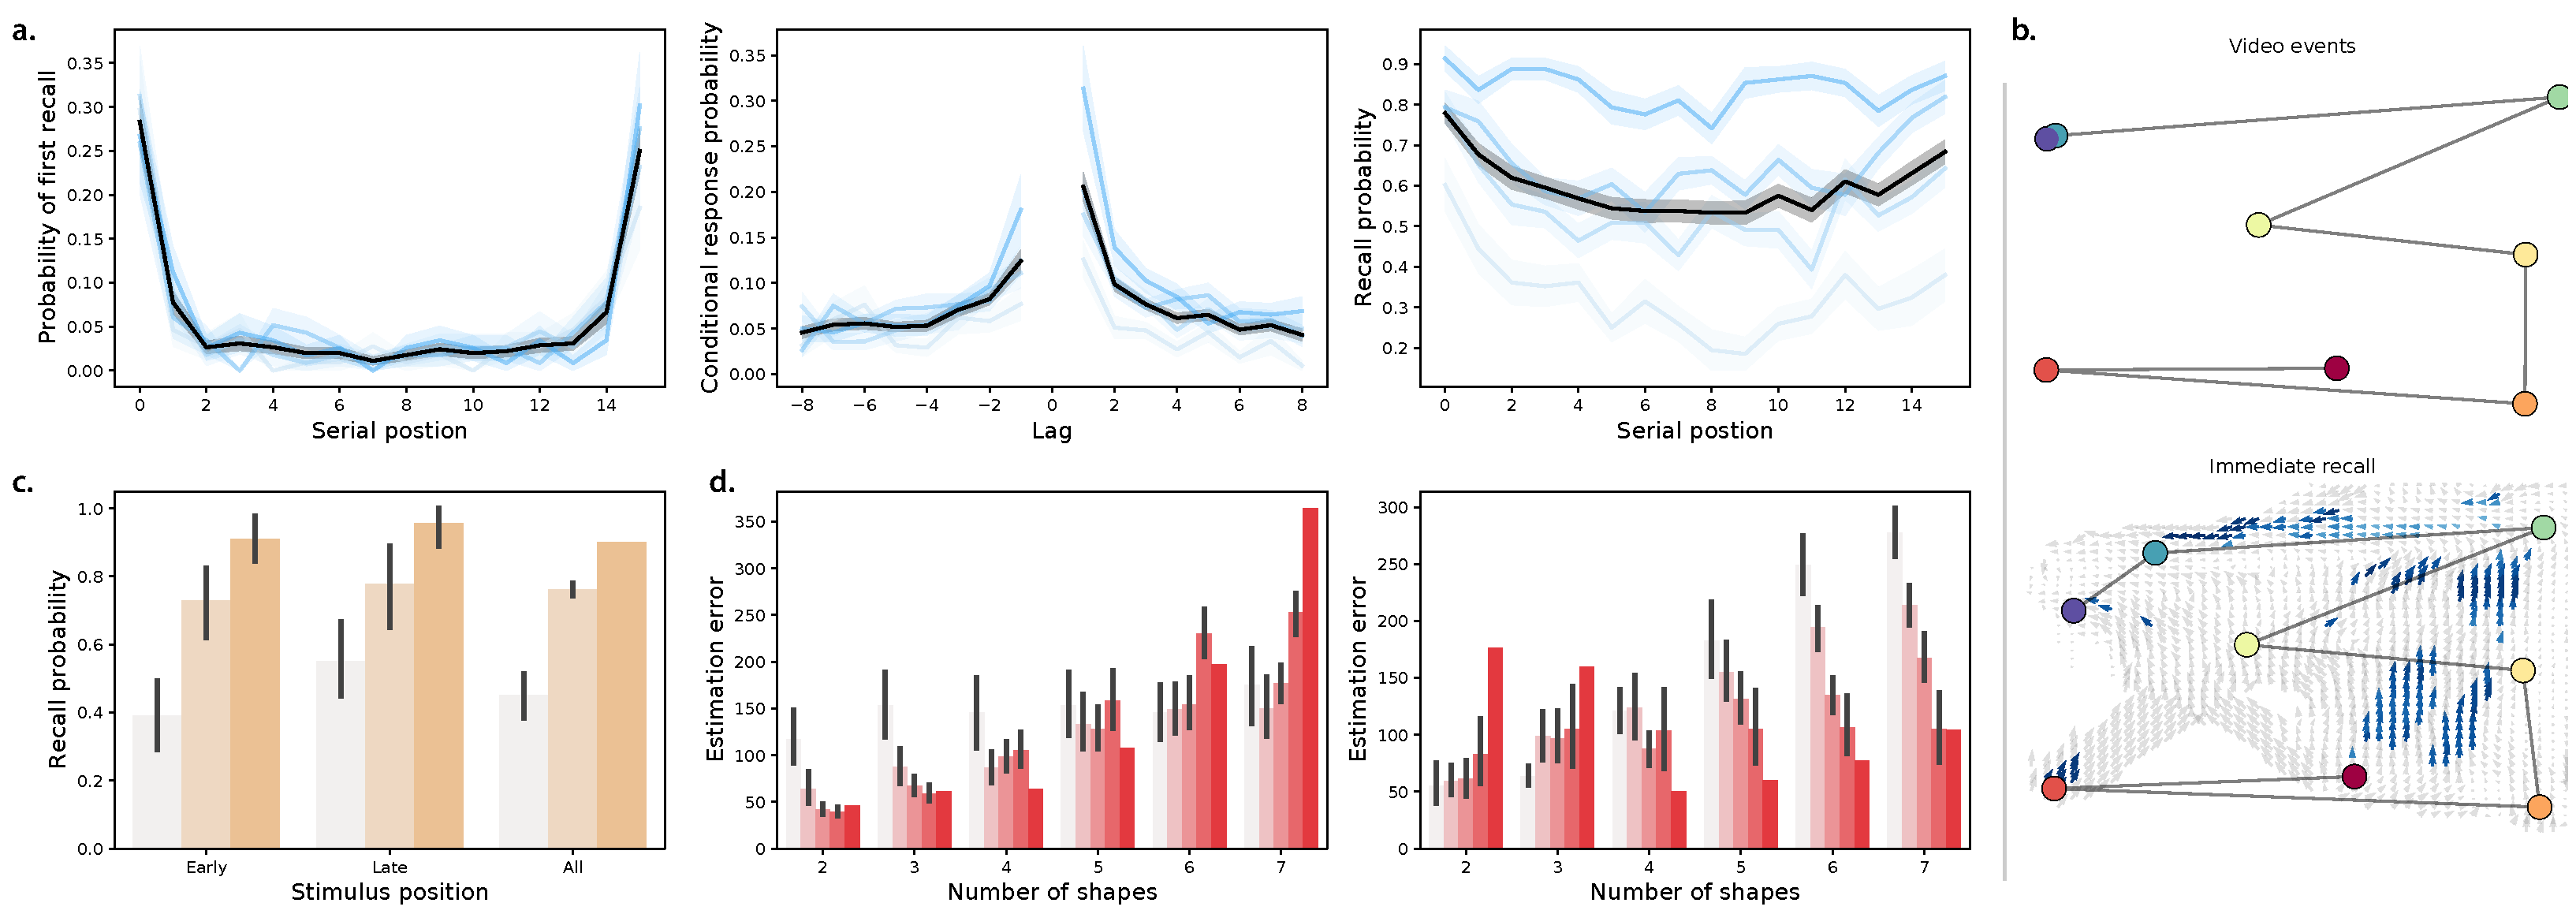
\includegraphics[width=1\textwidth]{figs/behavior_overview_immediate}
\caption{\textbf{Immediate memory tests.}  \textbf{a. Free recall.}
  Left: probability of recalling each word first as a function of its
  presentation position.  Middle: probability of transitioning between
successively recalling the word presented at position $i$, followed by
word presented at position $i + \mathrm{Lag}$.  Right: probability of
recalling each word as a function of its presentation position.  See
Figure~\frDetail~for additional details.
\textbf{b. Naturalistic recall.}  Top: 2D embedding of a 2.5~min video
clip; each dot reflects a narrative event (red denotes early events
and blue denotes later events).  Bottom: 2D embedding of the averaged
transcripts of participants' recountings of the narrative (dots: same
format as top panel).  The arrows denote the average trajectory
directions through the corresponding region of text embedding space,
for any participants whose recountings passed through that region.
Blue arrows denote statistically reliable agreement across
participants ($p < 0.05$, corrected).  See Figure~\natDetail~for
additional details.  \textbf{c. Foreign language
  flashcards.} Each bar denotes the average proportion of correctly
recalled Gaelic-English word pairs from early (first 3), late (last
3), or all (i.e., all 10) study positions.  See
Figure~\vocabDetail~for additional details.\textbf{d. Spatial
  learning.}  Average estimation error in shape locations as a
function of the number of shapes.  See Figure~\spatialDetail~for
additional details.  All panels: error bars and error
ribbons denote bootstrap-estimated 95\% confidence intervals.  Shading
(saturation) denotes results for different subsets of participants
assigned based on their task performance (Figs.~\frDetail,
\natDetail, \vocabDetail, and \spatialDetail~provide information about
which performance metrics and values the shading reflects; in general
more saturated colors denote participants who performed better on the
given task.)  In Panel d, participants are grouped in two ways; in the
left panel, participants are grouped according to the $y$-intercepts of regression lines (estimation error as a
function of the number of shapes); in the right panel, participants
are grouped according to the slopes of the same regression lines.}
\label{fig:immediate_behavior}
\end{figure}

\begin{figure}[tp]
\centering
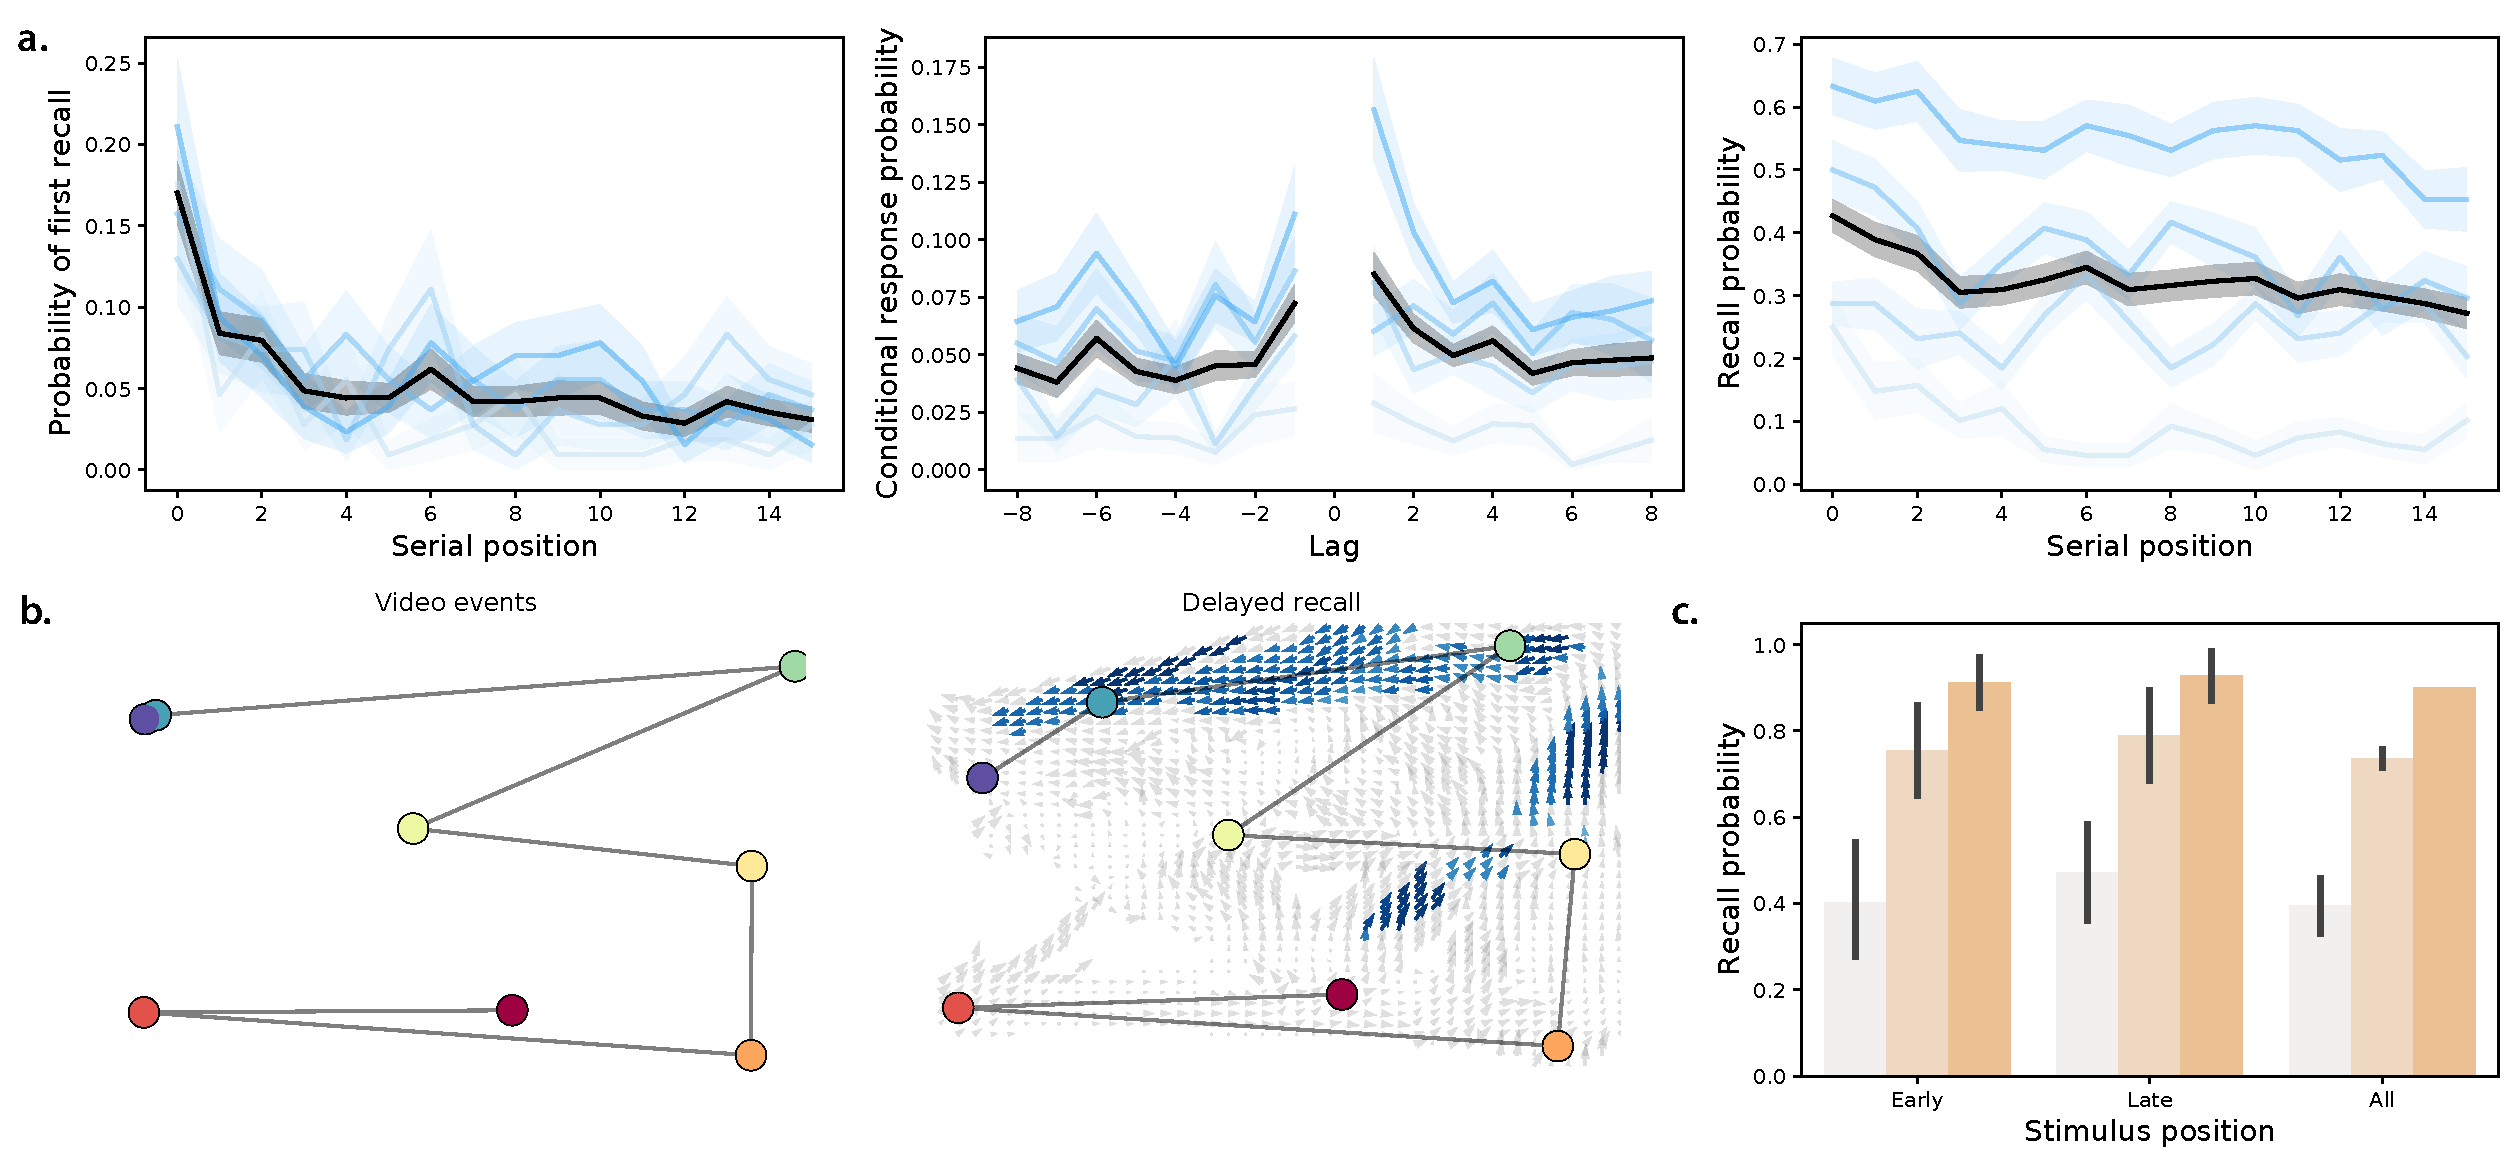
\includegraphics[width=1\textwidth]{figs/behavior_overview_delayed}
\caption{\textbf{Delayed memory tests.}  \textbf{a.  Free recall.}
  These panels are in the same format as
  Figure~\ref{fig:immediate_behavior}a, but they reflect performance
  on the delayed free recall task.  For additional details see
  Figure~\frDetail.  \textbf{b. Naturalistic recall.}  These panels
  are in the same format as Figure~\ref{fig:immediate_behavior}b, but
  the right panel reflects performance on the delayed naturalistic
  recall task.  For additional details see Figure~\natDetail.
  \textbf{c. Foreign language flashcards.} This panel is in the same
  format as Figure~\ref{fig:immediate_behavior}c, but it reflects
  performance on the delayed flashcards test.  For additional details
  see Figure~\vocabDetail.}
\label{fig:delayed_behavior}
\end{figure}

In addition to observing substantial across-participant variability in
memory performance, we also observed substantial variability in
participants' fitness and activity metrics
(Fig.~\ref{fig:fitness_summary}).  We examined recent measurements,
averaged over the week prior to testing
(Fig.~\ref{fig:fitness_summary}a), baselined measurements (average
over the prior week, divided by the average over the preceding 30 day;
Fig.~\ref{fig:fitness_summary}b), along with more gradually varying
measures that tended to remain relatively static over timescales of
weeks to months (Fig.~\ref{fig:fitness_summary}c).
Figure~\fitDists~displays across-participant
distributions for a broad selection of these measures, and Figures~\fitDistgridImmediate,
\fitScatterImmediate, \fitDistgridDelayed, and \fitScatterDelayed~show
different participants' fitness metrics, broken down by their
performance on different memory tasks.

\begin{figure}[tp]
\centering
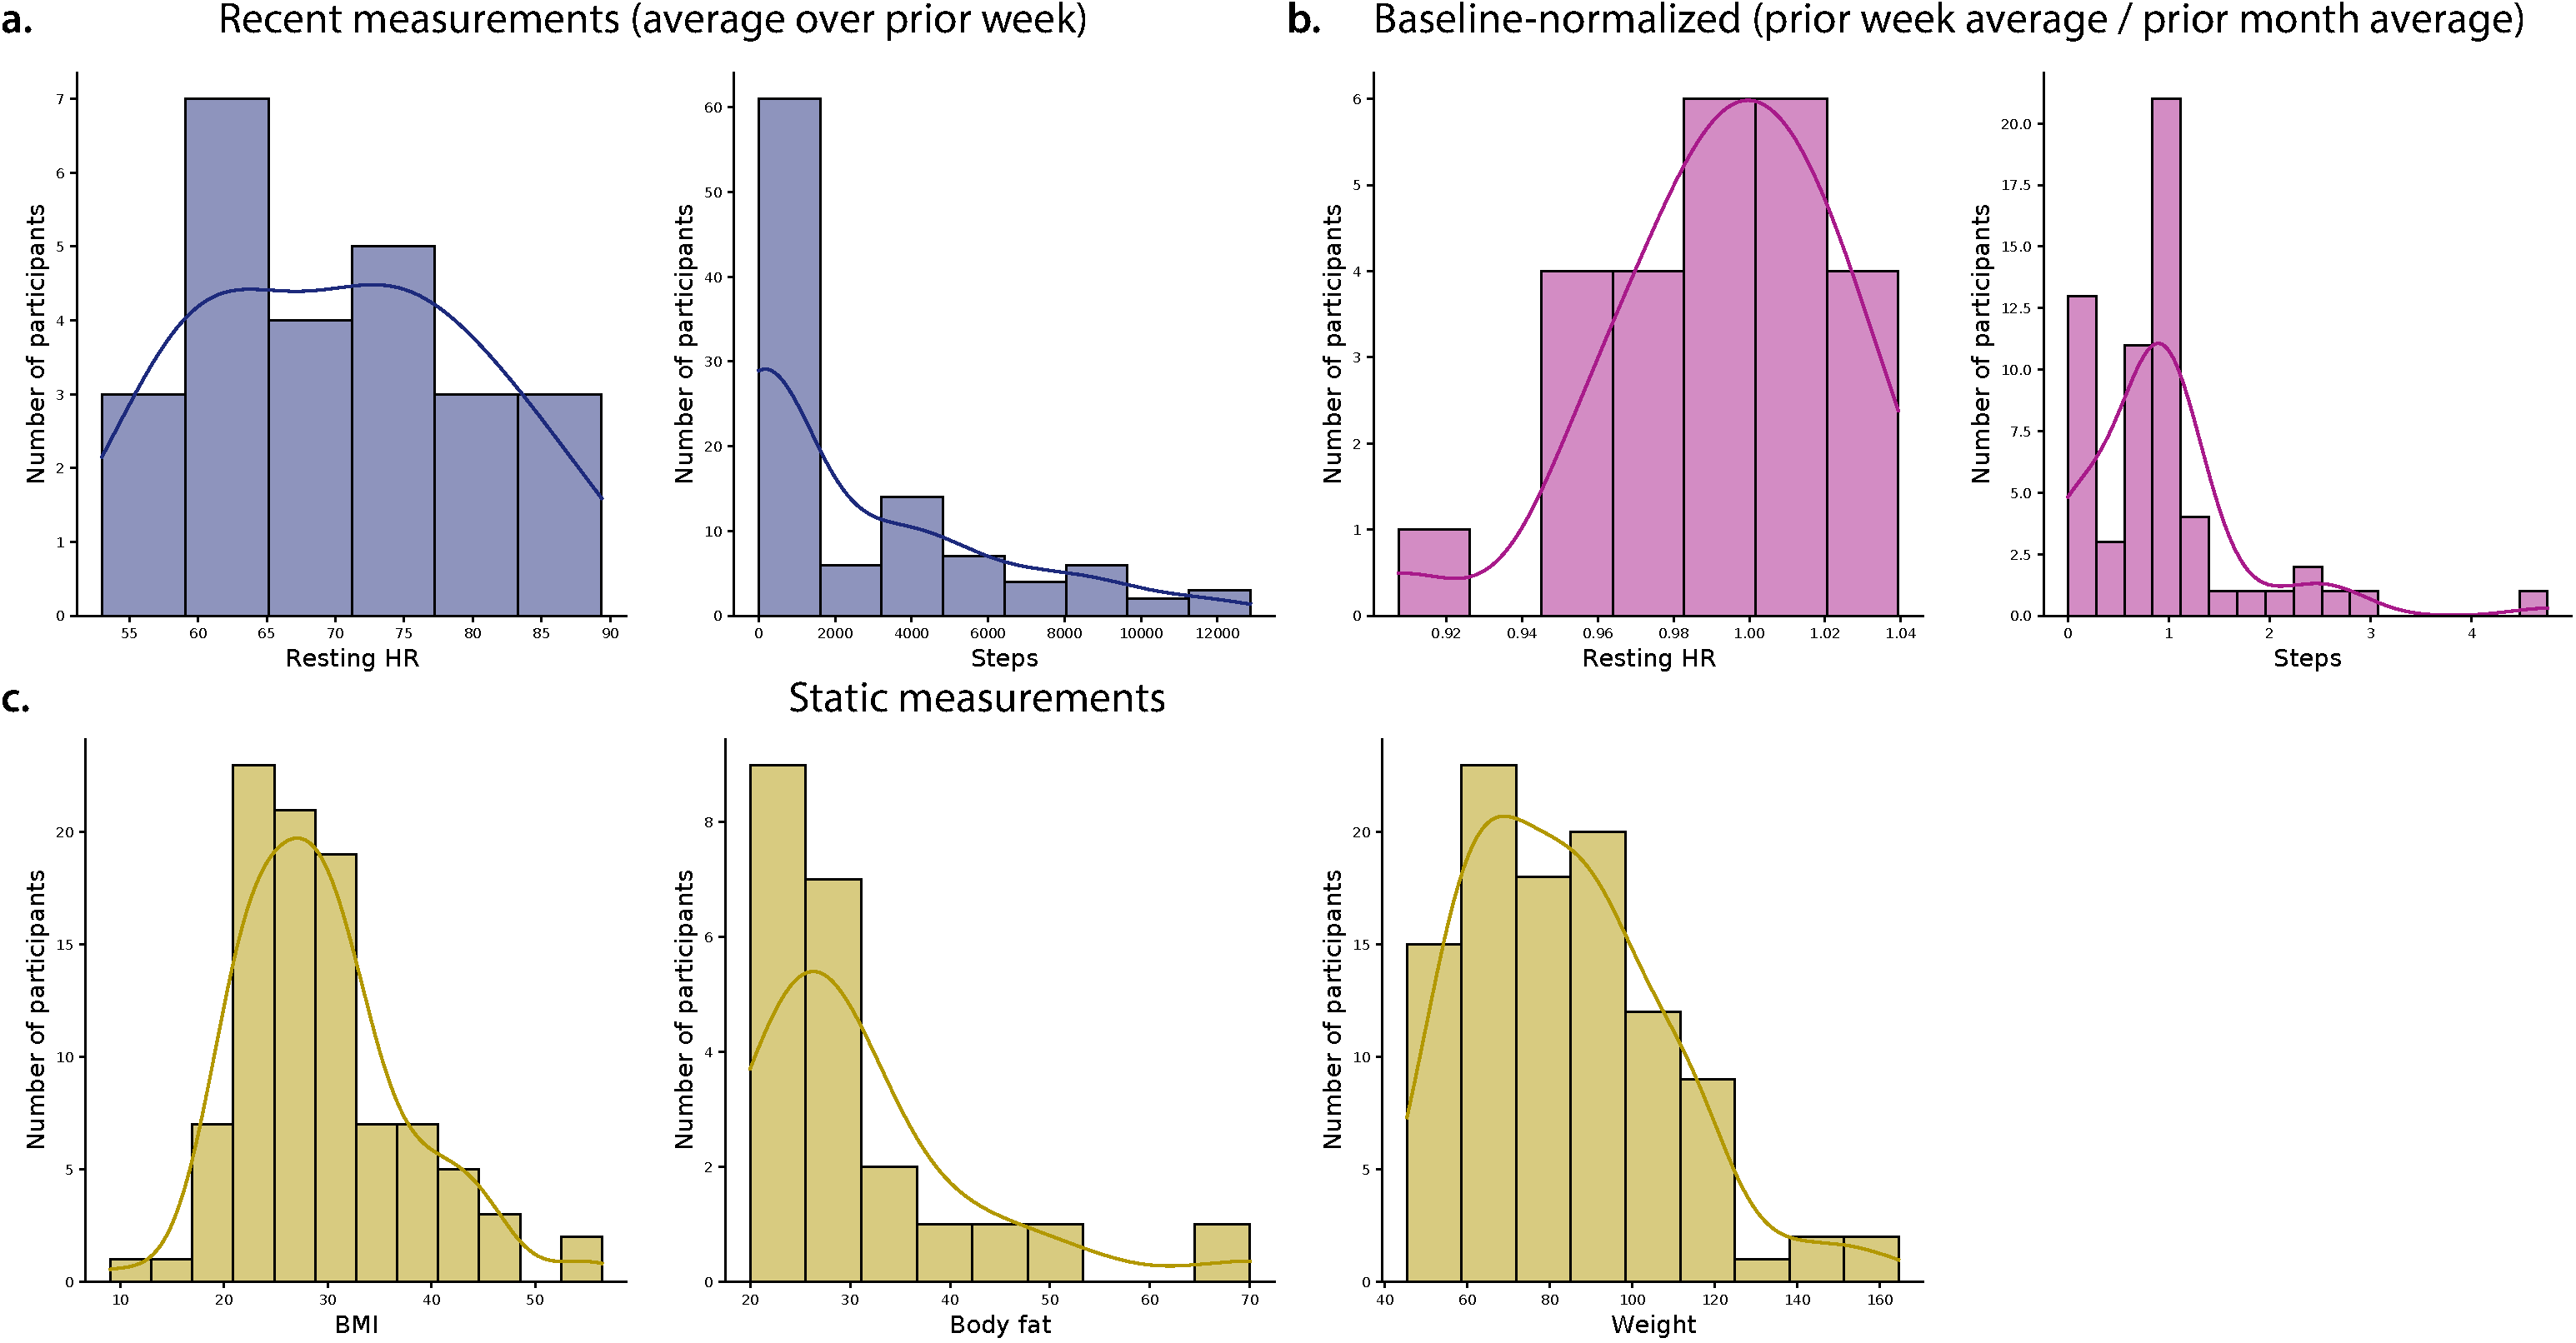
\includegraphics[width=0.8\textwidth]{figs/fitness_distributions_summary}
\caption{\textbf{Fitness measures.}  \textbf{a. Recent measures.}
  Resting heart rate (HR) and daily step counts, averaged over the
  week prior to testing.  \textbf{Baseline-normalized measures.}
  Resting heart rate and daily step counts averaged over the week
  prior to testing, divided by the average resting heart rate and step
counts averaged over the preceding month.  \textbf{Static measures.}
Body mass index (BMI), body fat percentage, and weight (in kg).  For
more information see Figures~\fitDists, \fitDistgridImmediate,
\fitScatterImmediate, \fitDistgridDelayed, and \fitScatterDelayed.}
\label{fig:fitness_summary}
\end{figure}

We wondered about potential links between the different aspects of
participants' data.  For example, if people who exercised in a
particular way also tended to perform better on a given memory task,
this could suggest that either (a) some property intrinsic to participants who
exercised in a particular way might also affect their memory
performance on the given task, and/or (b) particular exercise behaviors
could have a causal impact on memory performance.  We carried out an
exploratory analysis whereby we used a bootstrap-based approach (see
\textit{Exploratory correlation analyses}) to
identify reliable correlations between different aspects of memory
performance (Fig.~\behBehCorr), different aspects of fitness (Fig.~\fitFitCorr), different demographic
attributes (Fig.~\demDemCorr), and correlations between memory
performance, fitness information, and demographic attributes
(Fig.~\allCorr).  Several patterns emerged.  First, we found that
participants' performance on the (within-task) immediate versus delayed memory tests
from the free recall, naturalistic recall, and foreign language
flashcards tasks were positively correlated ($r$s $> 0.25$, $p$s $< 0.05$,
bootstrap corrected).  This suggests that, within each of these tasks,
similar processes or constraints may influence both short term and
long term information retrieval.  We also found reliable across-task correlations
between participants' (immediate and delayed) performance on the free
recall and foreign language flashcards tasks ($r$s $> 0.3$, $p$s $< 0.05$,
bootstrap corrected).

A large number of fitness-related measures displayed reliable
correlations (for a complete report, see Fig.~\fitFitCorr).  For
example, body mass index (BMI) and weight were correlated
($r = 0.91, p < 0.05$, bootstrap corrected).  Resting heart rate over
the prior week was negatively correlated with recent high-intensity
activity levels ($r = 0.39, p < 0.05$, bootstrap corrected).
Participants' peak heart rate (averaged over the prior week) were also
negative correlated with recent decreases in step counts and daily
elevation gains ($r\mathrm{s} < -0.27, p\mathrm{s} < 0.05$, boostrap
corrected), where recent changes were defined as the average values
over the seven days leading up to the test day divided by the average
values over the preceding 30 days.  Although several demographic
attributes (Fig.~\demDemCorr) displayed trivial correlations (e.g.,
participants identifying as male never reported identifying as female,
and so on), we also observed a negative correlation between reported
stress and alertness ($r = -0.44, p < 0.05$, bootstrap corrected), and
positive correlations between the reported task difficulties for all
tasks ($r\mathrm{s} > 0.26, p\mathrm{s} < 0.05$, bootstrap corrected).

We also found reliable correlations between participants' fitness and
demographic measures and their behaviors in different tasks
(for a complete report, see Fig.~\allCorr).  For example, recent
low-intensity (``fat burn'') cardiovascular activity was positively
correlated with immediate
($r = 0.44, p < 0.05$, bootstrap corrected) and delayed ($r = 0.37, p
< 0.05$, bootstrap corrected) recall on the naturalistic memory task.
Moderate intensity (``cardio'') cardiovascular activitiy was
positively correlated with immediate naturalistic recall ($r = 0.47, p
< 0.05$, bootstrap corrected) and immediate recall on the foreign
language flashcards task ($r = 0.43, p < 0.05$, bootstrap corrected).
Recent low-intensity (``out-of-range'') cardiovascular activity was
negatively correlated with spatial memory performance ($r = -0.31, p <
0.05$, bootstrap corrected) whereas recent high-intensity (``peak'')
cardiovascular activity was positively correlated with spatial memory
performance ($r = 0.34, p < 0.05$, bootstrap corrected).  Recent
increases in high-intensity cardiovascular activity (more activity
over the past 7 days than during the preceding 30 days) also predicted
spatial memory performance ($r = 0.41, p < 0.05$, bootstrap
corrected).  Coffee consumption was (slightly) positively correlated with
immediate free recall performance ($r = 0.17, p < 0.05$, bootstrap
corrected) and (slightly) negatively correlated with immediate
naturalistic recall performance ($r = -0.16, p < 0.05$, bootstrap
corrected).

\begin{itemize}
% \item characterizing behaviors (color by quartile and continue the
%   color scheme in later figures-- hue reflects task, shading reflects
%   performance.  white outline means immediate, black outline means delayed)
%   \begin{itemize}
%   \item Free recall (immediate + delayed): pfr, lag-CRP, spc  (color:
%     recall performance).  
%     Figure~\ref{fig:fr_behavioral}.
%     \item Naturalistic recall (immediate + delayed): reproduce a version of the sherlock
%       movie/recall trajectories (color: mean precision).  Figure~\ref{fig:nat_behavioral}.
%     \item Foreign language flashcards (immediate + delayed):
%       p(correct) histogram (color: p(correct)).  Figure~\ref{fig:vocab_behavioral}.
%       \item Spatial learning: mean error by number of shapes (color:
%         intercept and slope of line fit to errors as a function of the number of
%         shapes).  Figure~\ref{fig:spatial_behavioral}.
%       \end{itemize}
%     \item Fitness info (break down by task performance, potentially
%       separately for each task); also separate out recent (raw) and
%       recent versus baseline -- color using same color scheme as
%       behavior figure
%       \begin{itemize}
%       \item activity (steps, zone minutes, floors/elevation)
%       \item resting heart rate
%         \item sleep
%         \end{itemize}
  % \item exploratory analysis (correlations).  Possibly make some sort of scatter matrix or pairplot-- rows/columns:
  %         tasks.  Diagonal: histogram of performance metric for that
  %         task.  Above-diagonal entries: compare performance across
  %         tasks (by subject).  Below-diagonal entries: empty?
  %         density/2d histograms?
  %   \begin{itemize}
  %   \item Memory-memory
  %   \item fitness-fitness
  %   \item survey-survey
  %   \item (fitness + survey)-memory
  %   \end{itemize}
  \item predictive analysis (regressions)
    \begin{itemize}
    \item Predict memory performance on held-out task from other tasks
    \item Predict memory performance on each task using fitness data
      \item Predict memory performance on each task using survey data
      \end{itemize}
    \item Reverse correlations: look at recent changes versus baseline
      trends (color using same scheme as behavior figures).  Possibly 
      \begin{itemize}
      \item Fitness profile that predicts performance on each task (barplots + timelines)
      \item Fitness profile for each survey demographic (barplots + timelines)
        \begin{itemize}
          \item Select out mental health demographics (based on meds, stress levels)
          \end{itemize}
        \end{itemize}
  \end{itemize}

  \section*{Discussion}
  \begin{itemize}
  \item summarize key findings
  \item correlation versus causation
         \item what can vs. can't we know?  we can identify correlations, but not causal direction-- e.g. we cannot know whether exercise \textit{causes} mental changes versus whether people with particular neural profiles might tend to engage in particular exercise behaviors.  that being said, we \textit{can} separate out baseline tendencies (e.g., how people tend to exercise in general) versus recent changes (e.g., how they happened to have exercised prior to the experiment).
  \item related work (exercise/memory, exercise/mental health), what this study adds
    \item future direction: towards customized physical exercise recommendation engine for optimizing mental health and mental fitness
    \end{itemize}

   


\section*{Acknowledgements}
We acknowledge useful discussions with David Bucci, Emily Glasser,
Andrew Heusser, Abigail Bartolome, Lorie Loeb, Lucy Owen, and Kirsten
Ziman.  Our work was supported in part by the Dartmouth Young Minds
and Brains initiative.  The content is solely the responsibility of
the authors and does not necessarily represent the official views of
our supporting organizations.  This paper is dedicated to the memory
of David Bucci, who helped to inspire the theoretical foundations of
this work.  Dave served as a mentor and colleague on the project prior
to his passing.


\section*{Data and code availability}
All analysis code and data used in the present manuscript may be found
\href{https://github.com/ContextLab/brainfit-paper}{\underline{here}}.

\section*{Author contributions}
Concept: J.R.M.  Experiment implementation and data collection: G.M.N.
Analyses: G.M.N., E.C., P.C.F., and J.R.M.  Writing: J.R.M.

\section*{Competing interests}
The authors declare no competing interests.

\bibliographystyle{apa}
\bibliography{/Users/jmanning/CDL-bibliography/cdl}
\end{document}
